\section{Architektury informačních systémů}

\subsection{Přehled}

\textbf{Architektura informačního systému}: popis struktury a chování systému

\vspace{4pt}
\noindent Mezi základní složky informačního systému patří:
\begin{itemize}
    \item data, funkce, procesy (do\-ménově závislé, \textit{SaaS})
    \item technické detaily:
    \begin{itemize}
        \item software (\textit{PaaS})
        \item hardware (\textit{IaaS})
    \end{itemize}
\end{itemize}

\noindent Popis architektury provedeme pomocí \textbf{jednotlivých modelů} (datový model, hierarchie funkcí, activity diagram, stavový diagram). \textbf{Struktura} je určena daty a funkcemi, \textbf{chování} procesy.

\begin{figure}[H]
    \centering
    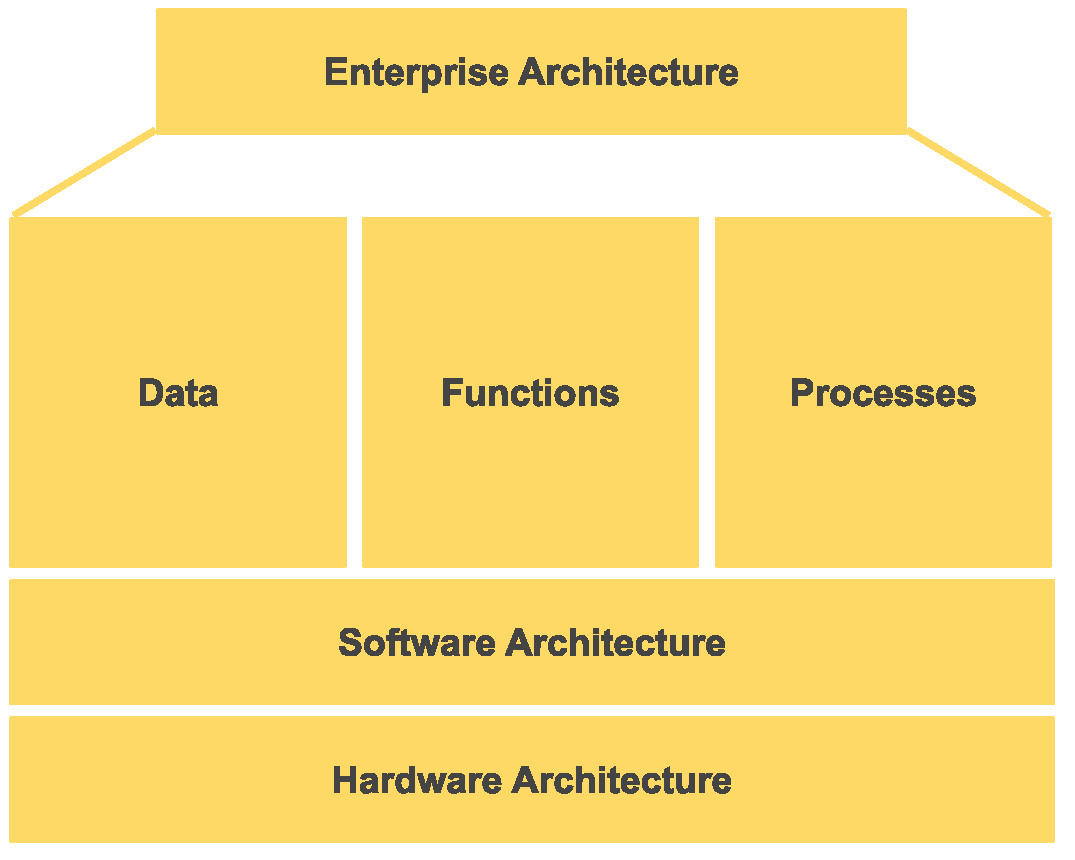
\includegraphics[width=.7\textwidth]{fig/02-architectures}
    \caption{Základní složky informačního systému}
\end{figure}

Vývojový koncept: návrh konceptu $\to$ obecný koncept $\to$ konkrétní implementace. To také závisí na \textbf{metodice} (analýza, návrh, implementace, testování, údržba) a \textbf{účastnících} (role: koncový uživatel, architekt, vývojář, administrátor).

\vspace{8pt}

\noindent \textbf{Enterprise architektura} se skládá z:
\begin{itemize}
    \item EIS (executive information systems) -- strategické rozhodování (např. dolování dat)
    \item BSS (business support systems) -- systémy na úrovni organizace (např. oddělení financí)
    \item OSS (operational support systems) -- nejnižší úroveň, (např. systém pro kontrolu překročení limitu dat v telekomunikační síti)
\end{itemize}

\noindent a boční systémy OIS (správa dokumentů) a B2B (komunikace mezi firmami).

\vspace{8pt}
\noindent \textbf{Typy organizace}:
\begin{itemize}
    \item vendor \textit{(poskytovatel)} -- dodává aplikaci, produkt (product manager)
    \item supplier \textit{(dodavatel)} -- přizpůsobí produkt na míru (techničtí a solution architekti, adminové)
    \item customer \textit{(uživatel)} -- definuje požadavky
\end{itemize}

\vspace{8pt}

\noindent \textbf{Role architektů}:

\begin{itemize}
    \item technický architekt -- architektura na technické úrovni
    \item solution architekt -- souvisí s dodavatelem, navrhuje řešení na konkrétní technologii
    \item enterprise architekt -- na vysoké úrovni, znají architekturu aplikací na úrovni aplikační (procesy, datové modely)
\end{itemize}

\subsection{Funkce a procesy}

\noindent \textbf{Klasifikace procesů}:

$\to$ Level 0 \textit{(business funkce)} -- správa zákazníků

$\to$ Level 1 \textit{(skupiny procesů)} -- správa operací zákazníků

$\to$ Level 2 \textit{(core business procesy)} -- správa objednávek

$\to$ Level 3 \textit{(business aktivity)} -- vytvoření objednávky, uzavření objednávky

$\to$ Level 4 \textit{(business task)} -- vyúčtování objednávky

$\to$ Level 5 \textit{(business step)} \ldots

\begin{figure}[H]
    \centering
    
\includegraphics[width=\textwidth]{fig/02-order-to-cash}
    \caption{Order to Cash proces u telekomunikačního operátora}
\end{figure}

\subsection{Data}

\textbf{Syntaxe}: datový formát, reprezentace, serializace

$\to$ \underline{XML, JSON}, objektivní datové modely, SQL, YAML \ldots

$\to$ musíme provést validaci, máme zde ale nástroje (XSL, schémata)

\vspace{4pt}

\noindent \textbf{Sémantika}: význam dat v rámci domény, ve které jsou použity, chápeme ji jak přirozeným jazykem, tak skrze data a strukturu.

\subsection{Integrace aplikací}

Existuje integrace vnitropodniková (SOA) a integrace mezi podniky (B2B). Klíčem k integraci je \textbf{rozhraní}, to se opět skládá z:

\begin{itemize}
    \item data -- vstup, výstup, struktury pro popis chybových zpráv
    \item funkce -- operace
    \item procesy -- veřejný proces \textit{("návod k použití", stavový diagram)}
    \item technické aspekty -- IP adresa, protokol
\end{itemize}

\subsection{Softwarové architektury}

Existuje více úrovní, na kterých rozhraní fungují:

$\to$ DBMS (data, funkce, procesy)

$\to$ JDBC

$\to$ JDO \textit{(Java třídy na data objekty)}

$\to$ Domain Object Model

\subsubsection*{Separation of Concerns}

Při vytváření aplikace můžu mít více vrstev (klient, server; nebo dvě rozdílné komponenty), je třeba se domluvit na rozhraní mezi jednotlivými vrstvami \textit{(manipulace s daty, integrita dat)}, jednotlivé vrstvy musí být nezávislé.

\subsubsection*{Client-server}

\begin{itemize}
    \item centrální server, skupina klientů
    \item monolitická / dvojvrstvá / třívrstvá \ldots
    \item \textbf{single point of failure} = pokud server vypadne, máme problém
    
    $\to$ proto zavedeny ochranné mechanismy
\end{itemize}

\subsubsection*{Peer-to-Peer}

\begin{itemize}
    \item spolehlivý (když uzel selže, jiné uzly zaberou jeho funkci)
    \item škálovatelný (více uzlů sdílí zátěž -- messaging systémy v enterprise systémech)
\end{itemize}

\vspace{4pt}
\noindent Existuje více typů architektur:

\subsubsection*{Monolitická}

Všechny vrstvy na jednom počítači, nepřesnosné aplikace na specifický operační systém. Samostatné aplikace, minimální integrace, lokální úložiště dat.

\vspace{4pt}
\noindent Nevýhodou je složitá údržba a problémy s integritou dat, škálovatelností a výkonem.

\subsubsection*{Dvojvrstvá}

\begin{itemize}
    \item prezentační a aplikační vrstva jsou odděleny od datové vrstvy
    \item datová vrstva je na specifickém serveru
    \item více uživatelů, sdílejících databázi
    \item SQL + nativní aplikace
\end{itemize}

\noindent Nevýhodou je thick klient, který je náročný na údržbu a integrace na data.

\subsubsection*{Třívrstvá}

Každá vrstva je na specifickém zařízení (tenký klient, komunikuje přes protokol se serverem, ten komunikuje s databází). Ani to ale nestačí \ldots

\subsubsection*{Middleware}

Přidáváme další middleware vrstvy mezi klienta a server. Problémem je nutnost škálovat jako celek, proto přišla:

\subsubsection*{Architektura mikroslužeb}

Jednotlivé middlewary, aplikace a DB monolity se rozpadají na jednotlivé mikroslužby, které jde již dobře škálovat.

\subsection{Typy middlewarů}

\subsubsection*{Škálovatelnost}

Zajišťují škálovatelnost, messaging servery, load balancers, proxy servery, reverse proxy

\subsubsection*{Funkční}

Zajišťují více flexibilní integraci, repozitáře, mediátoři (datová/procesová/technická interoperabilita -- SOAP), monitorování

\subsubsection*{Bezpečnostní}

Firewally a Gateways
